\documentclass[12pt]{article}

\usepackage[margin=1in]{geometry}
\linespread{1.4}

\usepackage{amsthm}
\usepackage{color}
\usepackage{tikz-cd}
\usepackage{quiver}
\usepackage{mathtools}
\usepackage{bbm}
\usepackage[hidelinks]{hyperref}
\usepackage{stmaryrd}
\usepackage{graphicx}
\usepackage{amssymb}
\usepackage{svg}

\usepackage{listings}
\usepackage{jlcode}

\usepackage[theorems]{tcolorbox}
\tcbuselibrary{breakable, theorems, skins}



\raggedbottom
\def\footnoterule{\vfill % added this
   \kern-3pt\hrule width 2truein \kern 2.6pt} % the \hrule is .4pt high





%\theoremstyle{definition}
%\newtheorem{definition}{Definition}

%\newtheorem{theorem}{Theorem}[section]


\definecolor{dodgerblue}{rgb}{0.12, 0.56, 1.0}
\definecolor{heliotrope}{rgb}{0.88,0.30,1.00}
\newcounter{examp}

\newtcbtheorem{example}{Example}{
    enhanced, before title={\stepcounter{examp}}, colback=blue!10, colframe=blue!35!black,
    fonttitle=\bfseries, before skip = 16pt, after skip = 16pt, attach boxed title to top left = {xshift=5mm, yshift*=-\tcboxedtitleheight/2},
    boxed title style = {colback=blue!35!black}}
{example}

\newtcbtheorem{definition}{Definition}{
    enhanced, before title={\stepcounter{examp}}, colback=dodgerblue!10, colframe=dodgerblue!35!black,
    fonttitle=\bfseries, before skip = 16pt, after skip = 16pt, attach boxed title to top left = {xshift=5mm, yshift*=-\tcboxedtitleheight/2},
    boxed title style = {colback=dodgerblue!35!black}}
{definition}

\newtcbtheorem{proofbox}{Proof}{
    enhanced, before title={\stepcounter{examp}}, colback=heliotrope!10, colframe=heliotrope!35!black,
    fonttitle=\bfseries, before skip = 16pt, after skip = 16pt, attach boxed title to top left = {xshift=5mm, yshift*=-\tcboxedtitleheight/2},
    boxed title style = {colback=heliotrope!35!black}}
{proofbox}



\title{Modeling Open Systems with Category Theory}
\author{Daniel Sinderson}
\date{May 2024}

\begin{document}
\maketitle


%%%%%%%%%%%%%%%%%%%%%%%%%%%%%%%%%%%%%
%%%%%%%%%%%%%%%%%%%%%%%%%%%%%%%%%%%%%
\section*{Introduction}
%%%%%%%%%%%%%%%%%%%%%%%%%%%%%%%%%%%%%
%%%%%%%%%%%%%%%%%%%%%%%%%%%%%%%%%%%%%
Category theory studies composition.
By studying and abstracting notions of composition, categories manage to encapsulate
a shockingly flexible and wide-reaching language for describing and working with structure of all sorts \cite{fong2019invitation}.
Much of modern mathematics, from vector spaces to groups, can be formalized in category theory.
Unlike with set theory though, this formalization is from a bird's eye point of view:
the details of a particular field go out of focus and only its high level structure remains \cite{riehl2017category}.
This is useful.
High levels of abstraction provide high levels of generality,
and a general, common language of how things are structured is useful for both organizing thought and sharing it.

Because of this generality, category theory also has some potential for reformulating difficult problems in other fields or even opening a broader class of phenomena to mathematical rigor.
This is an active field of research.
There are people using the tools of category theory to formalize and investigate everything from quantum mechanics and linguistics to logic and systems theory \cite{asudeh2020enriched, Coecke_Kissinger_2017, goldblatt2014topoi, myers2022categorical}.

It's this last application to systems theory that we will be looking more deeply at in this paper.
Though we are merely wandering at the edge of the work being done, we will see how to use category theory to build the specifications for, and simulate the behaviors of, dynamical systems built from the composition of smaller, simpler systems.
We will do this by modeling a gene transcription network as the composition of individual differential systems.
With even this introductory view of the subject matter it should be easy to see the promise of this approach to ease thinking about and designing models for large, complicated systems.






%\pagebreak
%%%%%%%%%%%%%%%%%%%%%%%%%%%%%%%%%%%%%
%%%%%%%%%%%%%%%%%%%%%%%%%%%%%%%%%%%%%
\section*{Category Theory Basics}
%%%%%%%%%%%%%%%%%%%%%%%%%%%%%%%%%%%%%
%%%%%%%%%%%%%%%%%%%%%%%%%%%%%%%%%%%%%
The first step to understanding category theory is to understand what a category is.
If you're new to higher mathematics, it's time to take a deep breath.
This will seem like a lot.

\begin{definition}{Category}{}
    A category $\mathcal{C}$ is defined by the following:
    \begin{enumerate}
        \item $\mathcal{C}$ contains a collection of objects $\mathsf{ob}(\mathcal{C})$. We will denote that an object is in a category using set notation: $c\in\mathcal{C}$.
        \item For any two objects $a$, $b$ $\in \mathcal{C}$ there is a collection of morphisms, or arrows, between those objects $\mathcal{C}(a,b)$ called the homset. This is short for ``set of homomorphisms.'' We will denote an element $f\in\mathcal{C}(a,b)$ using function notation: $f:a\rightarrow b$.
        \item Every object $a\in \mathcal{C}$ has a morphism to itself $\mathsf{id}_a:a\rightarrow a$ called its identity. This morphism doesn't do anything. It's like multiplying a number by 1.
        \item For every two morphisms $f:a\rightarrow b$ and $g: b\rightarrow c$ there's a third morphism $g\circ f:a\rightarrow c$ that is their composition. The circle is the symbol for function composition and $g \circ f$ is read ``g after f.''

              \[\begin{tikzcd}
                      a && b \\
                      \\
                      && c
                      \arrow["f", from=1-1, to=1-3]
                      \arrow["g", from=1-3, to=3-3]
                      \arrow["{g\circ f}"', from=1-1, to=3-3]
                  \end{tikzcd}\]

    \end{enumerate}
\end{definition}
\begin{definition*}{Category, cont.}{}
    These objects and morphisms are further constrained by the following properties:
    \begin{enumerate}
        \item (Unitality) Any morphism $f:a\rightarrow b$ can be composed with the identity morphisms of $a$ and $b$ such that $f\circ \mathsf{id}_a=\mathsf{id}_b\circ f=f$.

              \[\begin{tikzcd}
                      a && b
                      \arrow["{\mathsf{id}_a}"', from=1-1, to=1-1, loop, in=215, out=145, distance=10mm]
                      \arrow["f", from=1-1, to=1-3]
                      \arrow["{\mathsf{id}_b}", from=1-3, to=1-3, loop, in=325, out=35, distance=10mm]
                  \end{tikzcd}\]

        \item (Associativity) For any morphisms $f:a\rightarrow b$, $g:b\rightarrow c$, and $h:c\rightarrow d$, $h\circ (g\circ f)=(h\circ g)\circ f$. Since it doesn't matter what order we apply the morphisms, we write this $h\circ g \circ f$.

              \[\begin{tikzcd}
                      a & b & c & d
                      \arrow["f"', from=1-1, to=1-2]
                      \arrow["g"', from=1-2, to=1-3]
                      \arrow["h"', from=1-3, to=1-4]
                      \arrow["{{g\circ f}}", curve={height=-24pt}, from=1-1, to=1-3]
                      \arrow["{{h\circ g}}"', curve={height=24pt}, from=1-2, to=1-4]
                  \end{tikzcd}\]

    \end{enumerate}
\end{definition*}

Let's break this down a little bit.
We have a collection of objects with connections between them.
We know that every object is connected to itself.
And we know that if object $a$ is connected to $b$, and $b$ is connected to $c$, then $a$ is connected to $c$ through $b$.\footnote{For people with some background in math or logic this might be familiar as the transitive property.}

We also know that the objects and connections follow two rules.
First, that moving from an object to that same object doesn't do anything (unitality).
And second, that no matter how you group moving along connections it always amounts to the same trip (associativity).
That's it.
Categories are honestly pretty simple.
But from these humble beginnings we are going to climb very high.


\subsubsection*{A Quick Note on Isomorphism}
When most of us think of two things being ``the same'' in mathematics we think of equalities like $1 + 1 = 2$.
Equality is not the only useful notion of sameness in mathematics though.
When thinking about whether two objects in a category are meaningfully ``the same,'' a more useful notion than equality is that of isomorphism.
An isomorphism between objects means that, while they may not be exactly the same, as in equality, there exists a way to move between the two objects without losing any information.

\begin{definition}{Isomorphism}{}
    Two objects $a, b$ in a category are isomorphic if there exists a morphism $f:a\rightarrow b$ for which there is another morphism $f^{-1}:b\rightarrow a$ such that $f^{-1}\circ f=\mathsf{id}_a$ and $f\circ f^{-1}=\mathsf{id}_b$.
    Such a morphism is called an isomorphism.
    \[\begin{tikzcd}
            a && b
            \arrow["{\mathsf{id}_a}", from=1-1, to=1-1, loop, in=145, out=215, distance=10mm]
            \arrow["f", curve={height=-12pt}, from=1-1, to=1-3]
            \arrow["{{f^{-1}}}", curve={height=-12pt}, from=1-3, to=1-1]
            \arrow["{\mathsf{id}_b}"', from=1-3, to=1-3, loop, in=35, out=325, distance=10mm]
        \end{tikzcd}\]
\end{definition}

Another way to think about isomorphism is as a renaming.
Two objects are isomorphic if it's possible to represent one as the other by a simple, and reversible, relabeling.
For instance, an example of two sets that are isomorphic are the sets $\{a, b, c\}$ and $\{1, 2, 3\}$.
By relabeling $a \mapsto 1$, $b \mapsto 2$, and $c \mapsto 3$, we have represented the first set by means of the second set.
Specifically, we've labeled the first three letters of the alphabet by the numbers $1$, $2$, and $3$.


\subsection*{Functors and Categories of Categories}
Most mathematical structures have some way of mapping one instance of that structure to another instance.
Functions map sets to sets.
Linear transformations map vector spaces to other vector spaces.
And group homomorphisms map groups to other groups.
Since categories are a mathematical structure, it makes sense to ask if there exists a way to map between them.
Such a map would have to preserve all of the things that make a category a category: identity morphisms and composite morphisms, and the rules of unitality and associativity.
We call such a map between categories a functor.
\begin{definition}{Functor}{}
    A functor $F:\mathcal{C}\rightarrow\mathcal{D}$ is a map between categories $\mathcal{C}$ and $\mathcal{D}$ such that the following hold:
    \begin{enumerate}
        \item For any object $a\in\mathcal{C}$ there is an object $Fa\in\mathcal{D}$.
        \item For any morphism $f:a\rightarrow b$ between objects $a$ and $b$ in $\mathcal{C}$ there is a morphism $Ff:Fa\rightarrow Fb$ between objects $Fa$ and  $Fb$ in $\mathcal{D}$.
        \item For all objects $a\in\mathcal{C}$ and $Fa\in\mathcal{D}$, $F\mathsf{id}_a=\mathsf{id}_{Fa}$.
        \item For any composition of morphisms $g\circ f$ in $\mathcal{C}$, $F(g\circ f)=Fg\circ Ff$ in $\mathcal{D}$.
    \end{enumerate}
\end{definition}

There are some things to note here.
The first is that, like sets and functions, the mapping of objects from one category to another is unique.
Every object in the source category is mapped to exactly one object in the target category.
The same goes for morphisms.
The second thing to note is that identity morphisms get mapped to identity morphisms and compositions get mapped to compositions.

Let's check that these rules are enough to preserve unitality and associativity.
We will check unitality first.
\begin{proofbox}{Preservation of Unitality}{}
    Let a functor $F:\mathcal{C} \rightarrow \mathcal{D}$ be given, with objects $a,b\in\mathcal{C}$ and morphism $f:a \rightarrow b$.
    \begin{align*}
        F(\mathsf{id}_b \circ f) & = F\mathsf{id}_b \circ Ff   & \text{by the functor composition rule}   \\
                                 & = \mathsf{id}_{Fb} \circ Ff & \text{by the functor identity rule}      \\
                                 & = Ff                        & \text{by the definition of the identity} \\
                                 & = Ff \circ \mathsf{id}_{Fa} & \text{by the definition of the identity} \\
                                 & = Ff \circ F\mathsf{id}_a   & \text{by the functor identity rule}      \\
                                 & = F(f \circ \mathsf{id}_a)  & \text{by the functor composition rule}
    \end{align*}
    Thus the functor preserves unitality, since $F(\mathsf{id}_b \circ f) = F(f \circ \mathsf{id}_a) = Ff$. $\square$
\end{proofbox}
Now let's check that associativity is preserved.
\begin{proofbox}{Preservation of Associativity}{}
    Let a functor $F:\mathcal{C} \rightarrow \mathcal{D}$ be given, with objects $a,b,c,d\in\mathcal{C}$ and morphisms $f:a \rightarrow b$, $g:b \rightarrow c$, and $h:c \rightarrow d$.
    \begin{align*}
        F(h \circ (g \circ f)) & = Fh \circ F(g \circ f)  & \text{by the functor composition rule}                \\
                               & = Fh \circ (Fg \circ Ff) & \text{by the functor composition rule}                \\
                               & = (Fh \circ Fg) \circ Ff & \text{by associativity in the category $\mathcal{D}$} \\
                               & = F(h \circ g) \circ Ff  & \text{by the functor composition rule}                \\
                               & = F((h \circ g) \circ f) & \text{by the functor composition rule}
    \end{align*}
    Thus the functor preserves associativity, since $F(h \circ (g \circ f)) = F((h \circ g) \circ f)$. $\square$
\end{proofbox}

With functors in our toolbox, it's now possible to construct a category where the objects themselves are categories and the morphism between them are functors.
We call this category $\mathbf{Cat}$.
This, along with our next step, will prove to be extremely powerful.

\subsubsection*{A Quick Note on Avoiding Paradox}
For anyone who has taken a course in logic or set theory, that last paragraph might be ringing some alarm bells.
Whenever we have recursion in our structure like this, there's the opportunity for paradox to sneak in.
The category of categories is no exception.

To avoid the paradox of whether $\mathbf{Cat}$ contains itself, category theorists employ formal notions of ``size'' to differentiate distinct universes of categories or by invoking a seperation between sets and classes \cite{goldblatt2014topoi, riehl2017category}.
These formalisms can get pretty technical though, so we will be ignoring them in this paper.
For us it will be enough to assume that whenenever we talk about a category whose objects are also categories, our object categories are in some way ``smaller'' than the category that they're a part of, and thus of a different type.\footnote{In general, this ``smallness'' will be that the category's collection of objects forms a set, or that the homset between any two objects forms a set.}

\subsection*{Functor Categories and Natural Transformations}
For our next, and last, step up into abstraction let's talk about functor categories.
Functor categories are categories whose objects are functors and whose morphisms are maps called natural transformations.

Since natural transformations map functors to other functors, we know that they must preserve the essential ``functor-ness'' of functors.
This ``functor-ness'' is a bit harder to pin down than the ``category-ness'' that functors themselves preserve.
We need to see what natural transformations do to functors, but also what they do to the objects and arrows of the categories that the functors are acting on.

\begin{definition}{Natural Transformation}{}
    A natural transformation $\alpha :F\Rightarrow G$ is a map between functors $F:\mathcal{C}\rightarrow\mathcal{D}$ and $G:\mathcal{C}\rightarrow\mathcal{D}$ such that the following holds:
    \begin{enumerate}
        \item For each object $c\in\mathcal{C}$, there is a morphism $\alpha_c:Fc\rightarrow Gc$ in $\mathcal{D}$.
              These are called the component morphisms of $\alpha$.
        \item For every morphism $f:a\rightarrow b$ in $\mathcal{C}$, $\alpha_b\circ Ff=Gf\circ\alpha_a$.
              This is called the naturality condition, and it preserves functoriality.
    \end{enumerate}

    The naturality condition ensures that the following diagram commutes.
    \[\begin{tikzcd}
            Fa && Ga \\
            \\
            Fb && Gb
            \arrow["{\alpha_b}"', from=3-1, to=3-3]
            \arrow["Gf", from=1-3, to=3-3]
            \arrow["Ff"', from=1-1, to=3-1]
            \arrow["{\alpha_a}", from=1-1, to=1-3]
        \end{tikzcd}\]

    We can represent $\alpha$ diagramatically in the following condensed form.
    \[\begin{tikzcd}
            {\mathcal{C}} && {\mathcal{D}}
            \arrow[""{name=0, anchor=center, inner sep=0}, "F", curve={height=-18pt}, from=1-1, to=1-3]
            \arrow[""{name=1, anchor=center, inner sep=0}, "G"', curve={height=18pt}, from=1-1, to=1-3]
            \arrow["\alpha", shorten <=5pt, shorten >=5pt, Rightarrow, from=0, to=1]
        \end{tikzcd}\]


\end{definition}

This definition is short but there's a whole extra layer of stuff to keep track of since we added a layer of abstraction.
Let's get a better idea of what this definition captures by using a picture.\\

%\vspace*{0.25in}

%\includegraphics*[scale=0.75]{NT2.png}\\
\[\begin{tikzcd}
        {\mathcal{C}} &&& {\mathcal{D}} \\
        c &&& y \\
        &&&&& {\mathcal{C}} && {\mathcal{D}} \\
        b \\
        \\
        a &&& x
        \arrow[shift left, curve={height=-12pt}, dotted, from=2-1, to=2-4]
        \arrow[dashed, from=2-1, to=2-4]
        \arrow[""{name=0, anchor=center, inner sep=0}, "F", curve={height=-18pt}, from=3-6, to=3-8]
        \arrow[""{name=1, anchor=center, inner sep=0}, "G"', curve={height=18pt}, from=3-6, to=3-8]
        \arrow["g", from=4-1, to=2-1]
        \arrow[dotted, from=4-1, to=2-4]
        \arrow[dashed, from=4-1, to=6-4]
        \arrow["f", from=6-1, to=4-1]
        \arrow[dotted, from=6-1, to=6-4]
        \arrow[shift right, curve={height=12pt}, dashed, from=6-1, to=6-4]
        \arrow["k"', shift right, from=6-4, to=2-4]
        \arrow["\alpha", shorten <=5pt, shorten >=5pt, Rightarrow, from=0, to=1]
    \end{tikzcd}\]

\vspace*{0.25in}
Here we see two simple categories, $\mathcal{C}$ and $\mathcal{D}$, two functors $F$ (the dashed lines) and $G$ (the dotted lines) between them, and a natural transformation $\alpha$ that deforms $F$ into $G$.
Let's dig into this picture a bit and pick apart the functors and the natural transformation.

First, let's note all the important mappings of the functors and the component morphisms of the natural transformation.
\begin{align*}
    Fa=x             &  & Fb=x             &  & Fc=y          \\
    Ff=\mathsf{id}_x &  & Fg=k             &  & F(g\circ f)=k \\
                     &  &                  &  &               \\
    Ga=x             &  & Gb=y             &  & Gc=y          \\
    Gf=k             &  & Gg=\mathsf{id}_y &  & G(g\circ f)=k \\
\end{align*}
\begin{align*}
    \alpha_a:Fa\rightarrow Ga &  & \alpha_a = \mathsf{id}_x \\
    \alpha_b:Fb\rightarrow Gb &  & \alpha_b = k             \\
    \alpha_c:Fc\rightarrow Gc &  & \alpha_c = \mathsf{id}_y \\
\end{align*}


Next, let's check that the functors preserve composition.\footnote{You should be able to convince yourself that they preserve identities.}
$$F(g\circ f) = k = k \circ \mathsf{id}_x = Fg \circ Ff \ \ \ \ \checkmark$$
$$G(g \circ f) = k = \mathsf{id}_y \circ k = Gg \circ Gf \ \ \ \ \checkmark$$


And now let's look at the natural transformation $\alpha: F \Rightarrow G$ and make sure that it satisfies the naturality condition for the morphisms $f,g \in \mathcal{C}$.
$$\alpha_b \circ Ff = k \circ \mathsf{id}_x = Gf \circ \alpha_a \ \ \ \ \checkmark$$
$$\alpha_c \circ Fg = \mathsf{id}_y \circ k = Gg \circ \alpha_b \ \ \ \ \checkmark$$

Everything is working as expected.
Hopefully this helped to unpack some of the complexity behind the natural transformation definition.
In a real example, our functors would be defined equationally and we'd prove these properties for arbitrary morphisms instead of proving them for each morphism individually like we did here.


\subsection*{Duality}
The last thing we will cover in this section is the very simple, and very powerful, property of duality.
Every category has an opposite category that we write as $\mathcal{C}^{op}$.
The objects in this opposite category are exactly the same as in the original category, but every arrow is turned around: its source becomes its target and its target becomes its source.
Let's look at a simple example.\\\\
Let $\mathcal{C}$ be the category below.

\[\mathcal{C} := \begin{tikzcd}
        a && b && c \\
        \\
        && d && e
        \arrow[from=1-1, to=1-3]
        \arrow[from=1-1, to=3-3]
        \arrow[from=1-3, to=3-3]
        \arrow[from=3-3, to=3-5]
        \arrow[from=1-3, to=1-5]
        \arrow[from=1-5, to=3-5]
    \end{tikzcd}\]
\\\\It's opposite category, $\mathcal{C}^{op}$, is the following.
\[\mathcal{C}^{op} := \begin{tikzcd}
        a && b && c \\
        \\
        && d && e
        \arrow[from=1-3, to=1-1]
        \arrow[from=3-3, to=1-1]
        \arrow[from=3-3, to=1-3]
        \arrow[from=3-5, to=3-3]
        \arrow[from=1-5, to=1-3]
        \arrow[from=3-5, to=1-5]
    \end{tikzcd}\]
\\
And that's it.
One reason duality turns out to be so powerful is that it doubles our effectiveness.
For every structure in a category, we get the dual structure essentially for free \cite{cheng2022joy}.
Duality also plays an important role in representability and the Yoneda lemma which are major features of category theory that, unfortunately, we won't have space for in this paper.







%\pagebreak

%%%%%%%%%%%%%%%%%%%%%%%%%%%%%%%%%%%%%%%%%%%%
%%%%%%%%%%%%%%%%%%%%%%%%%%%%%%%%%%%%%%%%%%%%
\section*{Structure between Categories}
%%%%%%%%%%%%%%%%%%%%%%%%%%%%%%%%%%%%%%%%%%%%
%%%%%%%%%%%%%%%%%%%%%%%%%%%%%%%%%%%%%%%%%%%%
A category in isolation, like a set in isolation, doesn't give us much.
It's only when we begin adding relations and mappings between categories that the theory comes into its own.
These will include categorical versions of some familiar structures, like embeddings, equivalence relations, and isomorphisms.
But it will also include some structures that might seem strange and perplexing at first, like adjunctions and monads.


\subsection*{Subcategories}
Let's start with the simplest structure first, that of a subcategory relation.
Like any of the other ``sub-'' relations from other fields of mathematics, the subcategory relation encapsulates the notion of one category being in some way contained inside of another.
This means that the pattern of objects and morphisms that make up the subcategory are faithfully present in the other category.
Our first step will be to define this ``faithfulness.''

\begin{definition}{Faithful Functor}{}
    A functor $F:\mathcal{C}\rightarrow\mathcal{D}$ is faithful if for each $x,y\in\mathcal{C}$, the map $\mathcal{C}(x, y)\rightarrow\mathcal{D}(Fx,Fy)$ is injective.
\end{definition}
In other words, when a functor between categories is faithful, it means that every morphism between objects $x,y$ in the source category $\mathcal{C}$ is mapped to exactly one morphism between $Fx, Fy$ in the target category $\mathcal{D}$.
No morphisms in the source get collapsed into the same morphism in the target.
All of them are there.

However, this doesn't mean that objects can't be collapsed.
For that we need another condition on our functor.

\begin{definition}{Injective on Objects}{}
    A functor $F:\mathcal{C}\rightarrow\mathcal{D}$ is injective on objects if for each $x\in\mathcal{C}$, there is a unique $y\in\mathcal{D}$ such that $y=Fx$.
\end{definition}

With these two conditions we can define our subcategory relation.

\begin{definition}{Subcategory}{}
    A category $\mathcal{C}$ with a functor $F:\mathcal{C}\rightarrow\mathcal{D}$ that is both faithful and injective on objects is a subcategory of the category $\mathcal{D}$.
    A functor $F$ of this type is called an \textbf{embedding} of $\mathcal{C}$ into $\mathcal{D}$.
\end{definition}

Let's take a look at this using the two small categories below with a functor $F$ between them.

\[\begin{tikzcd}
        & {\mathcal{C}} &&& {\mathcal{D}} \\
        a & b && Fa & Fb \\
        & c & d && Fc & Fd & y
        \arrow["F", from=1-2, to=1-5]
        \arrow[from=2-1, to=2-2]
        \arrow[from=2-2, to=3-2]
        \arrow[from=2-2, to=3-3]
        \arrow[shift left, from=2-4, to=2-5]
        \arrow[shift right, from=2-4, to=2-5]
        \arrow[shift left=2, from=2-5, to=3-5]
        \arrow[shift right=2, from=2-5, to=3-5]
        \arrow[from=2-5, to=3-5]
        \arrow[from=2-5, to=3-6]
        \arrow[from=3-2, to=3-3]
        \arrow[from=3-5, to=3-6]
        \arrow[from=3-6, to=3-7]
    \end{tikzcd}\]

You should be able to convince yourself that $\mathcal{C}$ is a subcategory of $\mathcal{D}$ using the definitions of subcategory and functor above.
As expected we get injectivity on morphisms and objects.
But what if we also have surjectivity on morphisms?
To look into this let's define another property that a functor can have.

\begin{definition}{Full Functor}{}
    A functor $F:\mathcal{C}\rightarrow\mathcal{D}$ is full if for each $x,y\in\mathcal{C}$, the map $\mathcal{C}(x, y)\rightarrow\mathcal{D}(Fx,Fy)$ is surjective.
\end{definition}

This gives us a stronger version of the subcategory relation called a full subcategory that rejects any extraneous morphisms in the target category.

\begin{definition}{Full Subcategory}{}
    A category $\mathcal{C}$ with a functor $F:\mathcal{C}\rightarrow\mathcal{D}$ that is full, faithful, and injective on objects is a full subcategory of the domain $\mathcal{D}$.
    A functor $F$ of this type is called a \textbf{full embedding} of $\mathcal{C}$ into $\mathcal{D}$.
\end{definition}

Let's take a look at an example by paring down our category $D$ from the previous example.
\[\begin{tikzcd}
        & {\mathcal{C}} &&& {\mathcal{D}} \\
        a & b && Fa & Fb \\
        & c & d && Fc & Fd & y
        \arrow["F", from=1-2, to=1-5]
        \arrow[from=2-1, to=2-2]
        \arrow[from=2-2, to=3-2]
        \arrow[from=2-2, to=3-3]
        \arrow[from=2-4, to=2-5]
        \arrow[from=2-5, to=3-5]
        \arrow[from=2-5, to=3-6]
        \arrow[from=3-2, to=3-3]
        \arrow[from=3-5, to=3-6]
        \arrow[from=3-6, to=3-7]
    \end{tikzcd}\]

Again, convince yourself that this is indeed a full embedding.



\subsection*{Equivalence Relations between Categories}
Even more familiar than the subcategory relation, but less simple in the categorical context, are equivalence relations.
When comparing the ``sameness'' of categories there are several relations we can define.
In order of strictest to loosest these are equality, isomorphism, and equivalence.
Equality and isomorphism are actually quite simple.

\begin{definition}{Equality of Categories}{}
    Two categories are equal if they contain exactly the same objects and morphism.
\end{definition}

\begin{definition}{Isomorphism of Categories -- Subcategories}{}
    Two categories are isomorphic is they're both subcategories of each other.
\end{definition}
This is similar to the situation with sets where mutual subsets define an equality of sets.
By ensuring that every object and morphism in the source has a unique object and morphism in the target that it gets mapped to under the embedding $F:\mathcal{C} \rightarrow \mathcal{D}$ and vice versa under the embedding $G:\mathcal{D} \rightarrow \mathcal{C}$,
we ensure that our mappings between sets and objects are bijective and that our categories are isomorphic.

Another way to define an isomorphism between categories is as an isomorphism in the category of categories and functors, $\mathbf{Cat}$.
\begin{definition}{Isomorphism of Categories -- Category of Categories}{}
    Given two categories $\mathcal{C}, \mathcal{D} \in \textbf{Cat}$ and a pair of functors $F:\mathcal{C} \rightarrow \mathcal{D}$ and $G:\mathcal{D} \rightarrow \mathcal{C}$,
    $\mathcal{C}$ and $\mathcal{D}$ are isomorphic if $G \circ F = \mathsf{id_\mathcal{C}}$ and $F \circ G = \mathsf{id_\mathcal{D}}$.
\end{definition}


More useful than these is the notion of categorical equivalence and the notion of natural isomorphism that it relies on.

\begin{definition}{Natural Isomorphism}{}
    A natural isomorphism is a natural transformation $\alpha:F\Rightarrow G$ where all of the component morphisms of the transformation $\alpha_{c}:Fc\rightarrow Gc$ are isomorphisms.
\end{definition}

Let's try to get a handle on what this means by looking at the image we used to explore natural transformations.
\[\begin{tikzcd}
        {\mathcal{C}} &&& {\mathcal{D}} \\
        c &&& y \\
        &&&&& {\mathcal{C}} && {\mathcal{D}} \\
        b \\
        \\
        a &&& x
        \arrow[shift left, curve={height=-12pt}, dotted, from=2-1, to=2-4]
        \arrow[dashed, from=2-1, to=2-4]
        \arrow[""{name=0, anchor=center, inner sep=0}, "F", curve={height=-18pt}, from=3-6, to=3-8]
        \arrow[""{name=1, anchor=center, inner sep=0}, "G"', curve={height=18pt}, from=3-6, to=3-8]
        \arrow["g", from=4-1, to=2-1]
        \arrow[dotted, from=4-1, to=2-4]
        \arrow[dashed, from=4-1, to=6-4]
        \arrow["f", from=6-1, to=4-1]
        \arrow[dotted, from=6-1, to=6-4]
        \arrow[shift right, curve={height=12pt}, dashed, from=6-1, to=6-4]
        \arrow["k"', shift right, from=6-4, to=2-4]
        \arrow["\alpha", shorten <=5pt, shorten >=5pt, Rightarrow, from=0, to=1]
    \end{tikzcd}\]

\vspace*{0.25in}
As before, the components of $\alpha$ are the following:
$$\alpha_a = \mathsf{id}_x$$
$$\alpha_b = k$$
$$\alpha_c = \mathsf{id}_y$$
Our task now is to figure out which, if any, of these component morphisms are isomorphism.
For both identity morphisms the answer is yes: $\mathsf{id}_x \circ \mathsf{id}_x = \mathsf{id}_x$.
In general, if you do nothing and then do nothing again, you've still not done anything.\footnote{This is the kind of high-octane thinking that math opens up to us. Breathe it in.}
The case is different for $k$.
There simply is no morphism from $y$ to $x$ in $\mathcal{D}$ that could be the inverse of $k$, so $k$ cannot be an isomorphism.
This means our natural transformation $\alpha$ is not a natural isomorphism.

Let's make a small addition and try again.
\[\begin{tikzcd}
        {\mathcal{C}} &&& {\mathcal{D}} \\
        c &&& y \\
        &&&&& {\mathcal{C}} && {\mathcal{D}} \\
        b \\
        \\
        a &&& x
        \arrow[shift left, curve={height=-12pt}, dotted, from=2-1, to=2-4]
        \arrow[dashed, from=2-1, to=2-4]
        \arrow["{{k^{-1}}}"', shift right, from=2-4, to=6-4]
        \arrow[""{name=0, anchor=center, inner sep=0}, "F", curve={height=-18pt}, from=3-6, to=3-8]
        \arrow[""{name=1, anchor=center, inner sep=0}, "G"', curve={height=18pt}, from=3-6, to=3-8]
        \arrow["g", from=4-1, to=2-1]
        \arrow[dotted, from=4-1, to=2-4]
        \arrow[dashed, from=4-1, to=6-4]
        \arrow["f", from=6-1, to=4-1]
        \arrow[dotted, from=6-1, to=6-4]
        \arrow[shift right, curve={height=12pt}, dashed, from=6-1, to=6-4]
        \arrow["k"', shift right, from=6-4, to=2-4]
        \arrow["\alpha", shorten <=5pt, shorten >=5pt, Rightarrow, from=0, to=1]
    \end{tikzcd}\]

\vspace*{0.25in}
With this new diagram we've explicitly added an inverse of $k$, making it an isomorphism.
Since every component morphism of $\alpha$ is now an isomorphism, $\alpha$ itself is now a natural isomorphism.
With natural isomorphisms in hand we can define an equivalence between categories.
\begin{definition}{Categorical Equivalence}{}
    Two categories $\mathcal{C}$ and $\mathcal{D}$ are equivalent, written $\mathcal{C} \simeq \mathcal{D}$, if there exist two functors $F:\mathcal{C} \rightarrow \mathcal{D}$ and $G:\mathcal{D} \rightarrow \mathcal{C}$ with natural isomorphisms $\eta$ and $\epsilon$ such that $\eta : \mathsf{id}_\mathcal{C} \cong G \circ F$ and $\epsilon: \mathsf{id}_\mathcal{D} \cong F \circ G$.
\end{definition}
It might seem difficult to understand what's going on beneath this definition.
Let's try again using another property on functors.

\begin{definition}{Essentially Surjective Functor}{}
    A functor $F:\mathcal{C} \rightarrow \mathcal{D}$ is essentially surjective on objects if for every object $y \in \mathcal{D}$ there exists an object $x \in \mathcal{C}$ such that $Fx \cong y$.
\end{definition}

\begin{definition}{Categorical Equivalence, revisited}{}
    Two categories $\mathcal{C}$ and $\mathcal{D}$ are equivalent if there exists a functor $F$ between them that is faithful, full, and essentially surjective on objects.
\end{definition}

Let's look more deeply at this functor and what each of its properties guarantees.
Being essentially surjective on objects means that every object in our target category has some object from the source category that maps to it (up to isomorphism).
The combination of a full and faithful functor guarantees that for every set of morphisms between objects in our source category will be isomorphic to the set of morphisms between the image of those objects in the target category.
In other words, we have an isomorphism between morphisms and a surjection between objects (up to isomorphism).
If we look at our full subcategory example from above, are $\mathcal{C}$ and $\mathcal{D}$ equivalent?
\[\begin{tikzcd}
        & {\mathcal{C}} &&& {\mathcal{D}} \\
        a & b && Fa & Fb \\
        & c & d && Fc & Fd & y
        \arrow["F", from=1-2, to=1-5]
        \arrow[from=2-1, to=2-2]
        \arrow[from=2-2, to=3-2]
        \arrow[from=2-2, to=3-3]
        \arrow[from=2-4, to=2-5]
        \arrow[from=2-5, to=3-5]
        \arrow[from=2-5, to=3-6]
        \arrow[from=3-2, to=3-3]
        \arrow[from=3-5, to=3-6]
        \arrow[from=3-6, to=3-7]
    \end{tikzcd}\]
We know that $F$ is full and faithful by definition of a full subcategory.
But it's not surjective on objects since there's no object in $\mathcal{C}$ that maps to $y$, or anything isomorphic to $y$, in $\mathcal{D}$.
Let's make a quick modification so that our two categories can be equivalent.
\[\begin{tikzcd}
        & {\mathcal{C}} &&& {\mathcal{D}} \\
        a & b && Fa & Fb \\
        & c & d && Fc & Fd & y
        \arrow["F", from=1-2, to=1-5]
        \arrow[from=2-1, to=2-2]
        \arrow[from=2-2, to=3-2]
        \arrow[from=2-2, to=3-3]
        \arrow[from=2-4, to=2-5]
        \arrow[from=2-5, to=3-5]
        \arrow[from=2-5, to=3-6]
        \arrow[from=3-2, to=3-3]
        \arrow[from=3-5, to=3-6]
        \arrow[shift left, from=3-6, to=3-7]
        \arrow[shift left, from=3-7, to=3-6]
    \end{tikzcd}\]
Our collections of objects are now surjective up to isomorphism, so our functor is full, faithful, and essentially surjective and our two categories are equivalent.
Since categorical equivalence is an equivalence relation we know that the relation must be reflexive, symmetric, and transitive.
It's trivial to see that the relation is reflexive since the identity functor on a category meets all of our requirements, so we know a category is always equivalent to itself.
But how about symmetry?
Let's look at this using our example categories above and introduce a new functor $G$.
\[\begin{tikzcd}
        & {\mathcal{D}} &&& {\mathcal{C}} \\
        u & w &&& Gu & Gw \\
        & x & z & y && Gx & {Gy=Gz}
        \arrow["G", from=1-2, to=1-5]
        \arrow[from=2-1, to=2-2]
        \arrow[from=2-2, to=3-2]
        \arrow[from=2-2, to=3-3]
        \arrow[from=2-5, to=2-6]
        \arrow[from=2-6, to=3-6]
        \arrow[from=2-6, to=3-7]
        \arrow[from=3-2, to=3-3]
        \arrow[shift left, from=3-3, to=3-4]
        \arrow[shift left, from=3-4, to=3-3]
        \arrow[from=3-6, to=3-7]
    \end{tikzcd}\]
We can map $y$ and $z$ onto the same object $G$ and keep the functor essentially surjective.
But is it still full and faithful?
Naively we might think they aren't, since $\mathsf{id}_y$, $\mathsf{id}_z$, and both parts of the isomorphism between $y$ and $z$ all get mapped to $\mathsf{id}_{Gy}$, which certainly doesn't seem injective.
But $G$ is full and faithful.
Double checking that this is the case is a great opportunity to see why full and faithful functors are defined in terms of homsets.
\begin{proofbox}{$F$ is Full and Faithful}{}
    Given a functor $G: \mathcal{D} \rightarrow \mathcal{C}$ as defined above, for $G$ to be full and faithful there must be a bijection between the homset of any two objects in $\mathcal{D}$ and the homset of their images in $\mathcal{C}$.
    Since most of the objects and morphisms we are concerned with above obviously meet this requirement by inspection, let's focus on $y,z \in \mathcal{D}$ and the isomorphism between them, which we will call $f:y\rightarrow z$ and $f^{-1}:z\rightarrow y$, and their images.
    Listing them out, we have the following homsets.
    $$\mathcal{D}(y, y) = \{\mathsf{id}_y\} \cong \{\mathsf{id}_{Gy}\} = \mathcal{C}(Gy, Gy)$$
    $$\mathcal{D}(z, z) = \{\mathsf{id}_z\} \cong \{\mathsf{id}_{Gz}\} = \mathcal{C}(Gz, Gz)$$
    $$\mathcal{D}(y, z) = \{f\} \cong \{\mathsf{id}_{Gy}\} = \mathcal{C}(Gy, Gz)$$
    $$\mathcal{D}(z, y) = \{f^{-1}\} \cong \{\mathsf{id}_{Gz}\} = \mathcal{C}(Gz, Gy)$$
    So even though we have four morphisms that are all getting mapped to a single identity, each of the homsets individually is a singleton set in both the source and the target categories, meaning that they're all isomorphic, so our functor $G$ is indeed full and faithful. $\square$
\end{proofbox}

So we now know that categorical equivalence is reflexive and symmetric, but is it transitive?
To test this we will need another small category and another functor.
\[\begin{tikzcd}
        & {\mathcal{D}} &&& {\mathcal{E}} \\
        u & w &&& Gu & Gw & m \\
        & x & z & y && Gx & Gz & Gy
        \arrow["H", from=1-2, to=1-5]
        \arrow[from=2-1, to=2-2]
        \arrow[from=2-2, to=3-2]
        \arrow[from=2-2, to=3-3]
        \arrow[from=2-5, to=2-6]
        \arrow[shift left, from=2-6, to=2-7]
        \arrow[from=2-6, to=3-6]
        \arrow[from=2-6, to=3-7]
        \arrow[shift left, from=2-7, to=2-6]
        \arrow[from=3-2, to=3-3]
        \arrow[shift left, from=3-3, to=3-4]
        \arrow[shift left, from=3-4, to=3-3]
        \arrow[from=3-6, to=3-7]
        \arrow[shift left, from=3-7, to=3-8]
        \arrow[shift left, from=3-8, to=3-7]
    \end{tikzcd}\]
You should be able to convince yourself that $\mathcal{D}\simeq\mathcal{E}$ and that $\mathcal{C}\simeq\mathcal{E}$ using the same reasoning we used for our initial equivalence $\mathcal{C}\simeq\mathcal{D}$.

Since categorical equivalence is reflexive, symmetric, and transitive we know that it does define an equivalence relation.



\subsection*{Adjunctions}
Another important relationship that can exist between categories is an adjunction.
Adjunctions are a generalization of categorical equivalence.
Where an equivalence requires natural isomorphisms, an adjunction gets by with natural transformations.
What this means intuitively is that an adjunction is a way to encapsulate the notion of an imperfect inverse \cite{fong2019invitation}.
In an isomorphism or equivalence it's possible to move from one category to the other and then back and return to where you started (up to isomorphism of objects).
In an adjunction the guarantee is weaker: with each traversal an error accrues, but there is structure to it.

Let's look at this with an example using the two functions below.
\[\begin{tikzcd}
        {\mathbb{Z}} & {\mathbb{R}} && {\mathbb{R}} & {\mathbb{Z}} \\
        x & 2x && x & {\big\lceil \frac{1}{2}x \big\rceil}
        \arrow["f", from=1-1, to=1-2]
        \arrow[maps to, from=2-1, to=2-2]
        \arrow["g", from=1-4, to=1-5]
        \arrow[maps to, from=2-4, to=2-5]
    \end{tikzcd}\]
Here $f$ multiplies by 2 and $g$ divides by two and then rounds up to the nearest integer.
Let's throw in some values of $x$ and track it through our functions.
\begin{align*}
    g(f(3))=g(6)=3  &  & f(g(3))=f(2)=4 \\
    g(f(4))=g(8)=4  &  & f(g(4))=f(2)=4 \\
    g(f(5))=g(10)=5 &  & f(g(5))=f(3)=6
\end{align*}
Clearly these aren't isomorphisms: $f(g(x))$ isn't always equal to $x$ or to $g(f(x))$.
But the error is small and, more importantly, it's structured.
For any $x\in\mathbb{Z}$ and any $y\in\mathbb{R}$, $f(x) \le y$ if and only if $x \le g(y)$.
The specific structure here isn't important to us, only that there is one.

Let's make this precise now.
\begin{definition}{Adjunction}{}
    An adjunction between two categories $\mathcal{C}$ and $\mathcal{D}$ exists, written $\mathcal{C} \dashv \mathcal{D}$, if there exist two functors $F:\mathcal{C} \rightarrow \mathcal{D}$ and $G:\mathcal{D} \rightarrow \mathcal{C}$ with natural transformations $\eta : \mathsf{id}_\mathcal{C} \Rightarrow G \circ F$ and $\epsilon: F \circ G \Rightarrow \mathsf{id}_\mathcal{D}$ such that the following diagrams commute.
    \[\begin{tikzcd}
            F && {F \circ G \circ F} & G && {G \circ F \circ G} \\
            \\
            && F &&& G
            \arrow["{F \cdot \eta}", from=1-1, to=1-3]
            \arrow["{\epsilon \cdot F}", from=1-3, to=3-3]
            \arrow["{\mathsf{id}_F}"', from=1-1, to=3-3]
            \arrow["{\eta \cdot G}", from=1-4, to=1-6]
            \arrow["{G \cdot \epsilon}", from=1-6, to=3-6]
            \arrow["{\mathsf{id}_G}"', from=1-4, to=3-6]
        \end{tikzcd}\]
\end{definition}
You may have noticed there's something strange going on in the diagrams above.
Each of the objects is a functor and each of the morphisms is a natural transformation, but many of the morphisms appear to be the result of some kind of composition of a functor and a natural transformation.
This operation is called whiskering.
Whiskering is important for understanding the adjunction definition above and for understanding monads in the next section, so we will spend some time here to understand it.
\begin{definition}{Whiskering on the Right}{}
    Given functors $F,G: \mathcal{C} \rightarrow \mathcal{D}$ and $H:\mathcal{D} \rightarrow \mathcal{E}$ along with a natural transformation $\alpha:F \Rightarrow G$, if we whisker on the right we get a new natural transformation $H\cdot\alpha : (H \circ F) \Rightarrow (H \circ G)$ with components $(H\cdot\alpha)_a=H\alpha_a$.
    \[\begin{tikzcd}
            {\mathcal{C}} && {\mathcal{D}} & {\mathcal{E}} && {\mathcal{C}} &&& {\mathcal{E}}
            \arrow[""{name=0, anchor=center, inner sep=0}, "F", curve={height=-24pt}, from=1-1, to=1-3]
            \arrow[""{name=1, anchor=center, inner sep=0}, "G"', curve={height=24pt}, from=1-1, to=1-3]
            \arrow["H", from=1-3, to=1-4]
            \arrow[""{name=2, anchor=center, inner sep=0}, "{{H\circ F}}", curve={height=-24pt}, from=1-6, to=1-9]
            \arrow[""{name=3, anchor=center, inner sep=0}, "{{H \circ G}}"', curve={height=24pt}, from=1-6, to=1-9]
            \arrow["\alpha", shorten <=6pt, shorten >=6pt, Rightarrow, from=0, to=1]
            \arrow["H\cdot\alpha", shorten <=6pt, shorten >=6pt, Rightarrow, from=2, to=3]
        \end{tikzcd}\]
\end{definition}



\begin{definition}{Whiskering on the Left}{}
    Given functors $F: \mathcal{C} \rightarrow \mathcal{D}$ and $G,H:\mathcal{D} \rightarrow \mathcal{E}$ along with a natural transformation $\alpha:G \Rightarrow H$, if we whisker on the left we get a new natural transformation $\alpha\cdot F : (G \circ F) \Rightarrow (H \circ F)$ with components $(\alpha\cdot F)_a=\alpha_{Fa}$.
    \[\begin{tikzcd}
            {\mathcal{C}} & {\mathcal{D}} && {\mathcal{E}} && {\mathcal{C}} &&& {\mathcal{E}}
            \arrow["F", from=1-1, to=1-2]
            \arrow[""{name=0, anchor=center, inner sep=0}, "H"', curve={height=24pt}, from=1-2, to=1-4]
            \arrow[""{name=1, anchor=center, inner sep=0}, "G", curve={height=-24pt}, from=1-2, to=1-4]
            \arrow[""{name=2, anchor=center, inner sep=0}, "{G\circ F}", curve={height=-24pt}, from=1-6, to=1-9]
            \arrow[""{name=3, anchor=center, inner sep=0}, "{H \circ F}"', curve={height=24pt}, from=1-6, to=1-9]
            \arrow["\alpha", shorten <=6pt, shorten >=6pt, Rightarrow, from=1, to=0]
            \arrow["{\alpha \cdot F}", shorten <=6pt, shorten >=6pt, Rightarrow, from=2, to=3]
        \end{tikzcd}\]
\end{definition}
The results of this operation are easier to see if we look at the triangle diagrams above with the identity functors put in.
\[\begin{tikzcd}
        {F\circ \mathsf{id}_\mathcal{C}} && {F \circ G \circ F} & {\mathsf{id}_\mathcal{C} \circ G} && {G \circ F \circ G} \\
        \\
        && {\mathsf{id}_\mathcal{D} \circ F} &&& {G \circ \mathsf{id}_\mathcal{D}}
        \arrow["{F \cdot \eta}", from=1-1, to=1-3]
        \arrow["{\epsilon \cdot F}", from=1-3, to=3-3]
        \arrow["{\mathsf{id}_F}"', from=1-1, to=3-3]
        \arrow["{\eta \cdot G}", from=1-4, to=1-6]
        \arrow["{G \cdot \epsilon}", from=1-6, to=3-6]
        \arrow["{\mathsf{id}_G}"', from=1-4, to=3-6]
    \end{tikzcd}\]

Let's contrast our definition of adjunction to our definition of an isomorphism to help us get some intuition about how they work.
Given functors $F: \mathcal{C} \rightarrow \mathcal{D}$ and $G,H:\mathcal{D} \rightarrow \mathcal{E}$, we would have an isomorphism if $G \circ F = \mathsf{id}_\mathcal{C}$ and $F \circ G = \mathsf{id}_\mathcal{D}$.
But we don't have this in an adjunction.
Instead we have the natural transformations $\eta : \mathsf{id}_\mathcal{C} \Rightarrow G \circ F$ and $\epsilon: F \circ G \Rightarrow \mathsf{id}_\mathcal{D}$ and the triangle identities above.
At a high level, these tell us that--while the compositions don't equal the identities--there is still a way to travel from the identities on our categories to our compositions of functors.
This traveling accrues an error now though: it's no longer reversible.

%\begin{definition}[Adjunctions]
%    An adjunction between two categories $\mathcal{C}$ and $\mathcal{D}$ exists, written $\mathcal{C} \dashv \mathcal{D}$, if there exist two functors $F:\mathcal{C}\rightarrow\mathcal{D}$, the left adjoint functor, and $G:\mathcal{D}\rightarrow\mathcal{C}$, the right adjoint functor, such that for any object $c\in\mathcal{C}$ and any object $d\in\mathcal{D}$ there is a natural isomorphism $\mathcal{C}(c,Gd)\cong\mathcal{D}(Fc,d)$.
%\end{definition}
%In other words, $F$ and $G$ form an adjunction if the set of morphisms from $c$ to $Gd$ in $\mathcal{C}$ is isomorphic to the set of morphisms from $Fc$ to $d$ in $\mathcal{D}$.



\subsection*{Monads}
Our last relationship between categories, the monad, is explicitly a functor from a category to itself\footnote{When the domain and codomain of a functor are the same category we often call it an endofunctor.} rather than a relationship between arbitrary categories.
Like an adjunction though, a monad mutates the objects of the category it acts on in a non-reversible way: there's some loss of information that occurs that prevents an output from being uniquely identified with an input.
The connection between adjunctions and monads is actually quite deep.
But before we look into that, let's see the standard definition.
\begin{definition}{Monad}{}
    Given a category $\mathcal{C}$, a monad on $\mathcal{C}$ is a functor $M:\mathcal{C}\rightarrow\mathcal{C}$ with the following two natural transformations:
    \begin{enumerate}
        \item $\eta : \mathsf{id}_{\mathcal{C}} \Rightarrow M$ called the unit.
        \item $\mu: M\circ M \Rightarrow M$ called the multiplication.
    \end{enumerate}
    These natural transformation are required to make the following diagrams commute.

    \[\begin{tikzcd}
            M\circ M\circ M && M\circ M \\
            \\
            M\circ M && M
            \arrow["M\mu", from=1-1, to=1-3]
            \arrow["\mu", from=1-3, to=3-3]
            \arrow["\mu"', from=3-1, to=3-3]
            \arrow["{\mu M}"', from=1-1, to=3-1]
        \end{tikzcd}\]

    \[\begin{tikzcd}
            M && M\circ M && M \\
            \\
            && M
            \arrow["{\eta M}", from=1-1, to=1-3]
            \arrow["M\eta"', from=1-5, to=1-3]
            \arrow["\mu", from=1-3, to=3-3]
            \arrow["{\mathsf{id}_M}", from=1-5, to=3-3]
            \arrow["{\mathsf{id}_M}"', from=1-1, to=3-3]
        \end{tikzcd}\]

    For those with some experience with algebraic structures, this creates a monoidal structure on the collection of endofunctors $\{M, M\circ M, M\circ M\circ M,\dots\}$ where the monoidal unit is $\eta$ and the monoidal product is $\mu$.\footnote{This is the reason for the oft maligned phrase that ``monads are just monoids in the category of endofunctors.''}
\end{definition}

As we mentioned before there's a deep connection between adjunctions and monads.
Specifically, every adjunction gives rise to a monad $G \circ F: \mathcal{C} \rightarrow \mathcal{C}$ where $G$ is the right adjoint functor and $F$ is the left adjoint functor.
We can think of this induced monad as the impression or shadow left by the adjunction \cite{riehl2017category}.\footnote{Specifically the impression left on the codomain of the right adjoint.}
Looking at this more rigorously we can construct an alternate definition.

\begin{definition}{Monad Induced by an Adjunction}{}
    Every adjunction $F \dashv G$ induces a monad $G \circ F: \mathcal{C} \rightarrow \mathcal{C}$ where the unit is the natural transformation $\eta : \mathsf{id}_\mathcal{C} \Rightarrow G \circ F$ and the multiplication is the whiskered natural transformation $G \cdot \epsilon \cdot F: G \circ F \circ G \circ F \Rightarrow G \circ F$.
\end{definition}

Monads often show up in applied settings when the notion of a side-effect or additional structure on outputs is required.
In the context of categorical systems theory, monads make it possible to compose nondeterministic sytems.










%\pagebreak
%%%%%%%%%%%%%%%%%%%%%%%%%%%%%%%%%%%%%%%%%%%%%%%%%%%%%%%
%%%%%%%%%%%%%%%%%%%%%%%%%%%%%%%%%%%%%%%%%%%%%%%%%%%%%%%
\section*{Structure within Categories}
%%%%%%%%%%%%%%%%%%%%%%%%%%%%%%%%%%%%%%%%%%%%%%%%%%%%%%%
%%%%%%%%%%%%%%%%%%%%%%%%%%%%%%%%%%%%%%%%%%%%%%%%%%%%%%%

We will now look at the kinds of structures that we can find within a category.
We call these structures universal properties.
The general theory of universal properties is rich, but it's also very abstract and, unfortunately, outside of the scope of this paper \cite{riehl2017category}.
Instead, we will focus on two specific examples of a universal property that are important to the theory we explore later on: terminal objects and products.

\subsection*{Terminal Objects}
A terminal object in a category is an object that has exactly one morphism to it from every other object in the category.
It's the Rome of a category: all roads lead to it.

\begin{definition}{Terminal Object}{}
    Let $t\in\mathcal{C}$ be given. Then $t$ is a terminal object in $\mathcal{C}$ if the following hold:
    \begin{enumerate}
        \item For all $x\in\mathcal{C}$, there is exactly one morphism $f:x\rightarrow t$.
        \item For any other object $t'$ in $\mathcal{C}$ that meets condition (1), there exists a unique isomorphism $g:t\rightarrow t'$.
    \end{enumerate}
\end{definition}
Note here that a terminal object in a category is unique up to unique isomorphism and not strictly unique: as long as there's a unique isomorphism between them, there can be an infinite number of terminal objects in the category.
This is in fact the case in the category $\textbf{Set}$ of sets and functions where all singleton sets $\{*\}$ are terminal.
If we think about this it should make sense.
For any set $S$ there is exactly one function $f:S \rightarrow \{*\}$: the function that sends all elements in $S$ to $*$.
This includes any other singleton set $\{-\}$.
And since both singletons have the same cardinality and since $f$ is surjective we know that this one function between them is an isomorphism.

Also note that not every category has a terminal object.
For instance the category below has no object that has a morphism to it from every other object.
\[\begin{tikzcd}
        a & b \\
        c & d
        \arrow[from=1-1, to=1-2]
        \arrow[from=2-1, to=2-2]
    \end{tikzcd}\]
The existence of a terminal object is not a given in a category, but is structure that some categories have that tells us something about them.
The same is true for products.

\subsection*{Products}
Products in category theory are different than the products of two numbers that we are used to, though it is related in a very generalized way.
A product in a category is an object with morphisms from it to two other objects that is in some precise way the ``simplest'' or ``best'' such object.
This is vague, but take the product of integers $3*5=15$ as an example.
In this case, $15$ is the simplest number such that both $3$ and $5$ are among its divisors.
Contrast this to $30$ which does have $3$ and $5$ as divisors, but also $2$.
This extra divisor is superfluous and makes $30$ a worse candidate for $3*5$ than $15$.
Let's see this in diagram form.
\[\begin{tikzcd}
        && 30 \\
        \\
        && 15 \\
        \\
        3 &&&& 5
        \arrow["{x\div 2}", from=1-3, to=3-3]
        \arrow["{x \div 5}", from=3-3, to=5-1]
        \arrow["{x \div 3}"', from=3-3, to=5-5]
        \arrow["{(x\div 2)\div 3}", curve={height=-12pt}, from=1-3, to=5-5]
        \arrow["{(x\div 2)\div 5}"', curve={height=12pt}, from=1-3, to=5-1]
    \end{tikzcd}\]
Now let's make this precise in the general case.

\begin{definition}{Product}{}
    Let $a,b,v\in\mathcal{C}$ and morphisms $f:v\rightarrow a$ and $g:v\rightarrow b$ be given.
    \[\begin{tikzcd}
            & v \\
            a && b
            \arrow["f", from=1-2, to=2-1]
            \arrow["g"', from=1-2, to=2-3]
        \end{tikzcd}\]
    The object $v$ is a product of $a$ and $b$ if the following holds:
    \begin{itemize}
        \item For any other object $x$ with morphisms $f':x\rightarrow a$ and $g':x\rightarrow b$, there is a unique morphism $k:x\rightarrow v$ such that $f\circ k=f'$ and $g\circ k=g'$.
    \end{itemize}

    This means the following diagram commutes:
    \[\begin{tikzcd}
            & x \\
            & v \\
            a && b
            \arrow["f", from=2-2, to=3-1]
            \arrow["g"', from=2-2, to=3-3]
            \arrow["{g'}", curve={height=-12pt}, from=1-2, to=3-3]
            \arrow["{f'}"', curve={height=12pt}, from=1-2, to=3-1]
            \arrow["k", dashed, from=1-2, to=2-2]
        \end{tikzcd}\]

\end{definition}
This condition ensures that the object $v$ is the universal or canonical object satisfying the pattern, with the morphisms of any other such object being able to be written as a sort of embellishment of the morphisms from $v$.

In $\textbf{Set}$ the categorical product is exactly the Cartesian product of sets $a \times b = \{(x, y) \ | \ x\in a \text{ and } y\in b\}$, and $f$ and $g$ are the projections $f: (x, y) \mapsto x$ and $g: (x, y) \mapsto y$.
Like in our integer example above there are other candidates, say the object $(a \times b) \times c$, but all of these other candidates will have a unique factorization to the Cartesian product: they all have extra stuff.
Again we can see the example of $(a \times b) \times c$ in a diagram.
\[\begin{tikzcd}
        &&& {(a\times b) \times c} \\
        \\
        \\
        &&& {a \times b} \\
        \\
        a &&&&&& b
        \arrow["{((x, y), z) \mapsto (x,y)}", from=1-4, to=4-4]
        \arrow["{(x,y) \mapsto x}", from=4-4, to=6-1]
        \arrow["{(x,y) \mapsto y}"', from=4-4, to=6-7]
        \arrow["{((x, y), z) \mapsto (x,y) \mapsto y}", curve={height=-30pt}, from=1-4, to=6-7]
        \arrow["{((x, y), z) \mapsto (x,y) \mapsto x}"', curve={height=30pt}, from=1-4, to=6-1]
    \end{tikzcd}\]


It turns out that the category of categories also has products, and they are very similar to the cartesian product of sets or the external direct product of groups.

\begin{definition}{The Product of Categories}{}
    Given two categories $\mathcal{C}$ and $\mathcal{D}$, their product is a new category $\mathcal{C} \times \mathcal{D}$ defined as follows.
    \begin{enumerate}
        \item A collection of objects $(c, d)$ where $c\in\mathcal{C}$ and $d\in\mathcal{D}$.
        \item For any two objects $(c,d), (c',d') \in \mathcal{C} \times \mathcal{D}$, a collection of morphisms \\ $(f,g): (c,d) \rightarrow (c',d')$ where $f:c \rightarrow c'$ is a morphism in $\mathcal{C}$ and $g: d \rightarrow d'$ is a morphism in $\mathcal{D}$.
        \item Identity morphisms $\mathsf{id}_{(c,d)} = (\mathsf{id}_c, \mathsf{id}_d)$.
        \item And composition of morphisms done by composing the morphisms component-wise, so $(h,j) \circ (f,g) = (h\circ f, j \circ g)$.
    \end{enumerate}
\end{definition}

We can see how this is similar to the external direct product in the way that the structures are redefined component-wise, and thus how the product category inherits its structure from its underlying categories.
This product of categories is central to our next section.


%\pagebreak
%%%%%%%%%%%%%%%%%%%%%%%%%%%%%%%%%%%%%%%%%%%%%%
%%%%%%%%%%%%%%%%%%%%%%%%%%%%%%%%%%%%%%%%%%%%%%
\section*{Adding Structure to Categories}
%%%%%%%%%%%%%%%%%%%%%%%%%%%%%%%%%%%%%%%%%%%%%%
%%%%%%%%%%%%%%%%%%%%%%%%%%%%%%%%%%%%%%%%%%%%%%
The last piece of category theory we need before moving on to how this all relates to the theory of systems is the notion of a monoidal category.
Much like we can add additional structure on a set, we can do the same with a category.
For instance, if we take a set $S$ and add a binary operation $*:S \times S \rightarrow S$ that's associative and has a unit we get a structure called a monoid.
If we do something similar and slightly more complicated to a category, we get a monoidal category.

\begin{definition}{Monoidal Categories}{}
    A category $\mathcal{C}$ is monoidal if the following exist.
    \begin{enumerate}
        \item A functor $\otimes:\mathcal{C}\times\mathcal{C}\rightarrow\mathcal{C}$ called the monoidal product.
        \item An object $\mathbbm{1}\in\mathcal{C}$ called the unit.
        \item A natural isomorphism $\alpha : (a\otimes b)\otimes c\Rightarrow a\otimes (b\otimes c)$ called the associator, with components $\alpha_{x,y,z}: (x\otimes y)\otimes z\rightarrow x\otimes (y\otimes z)$.
        \item A natural isomorphism $\lambda : \mathbbm{1}\otimes a\Rightarrow a$ called the left unitor with components $\lambda_x : \mathbbm{1}\otimes x\rightarrow x$.
        \item A natural isomorphism $\rho : a\otimes \mathbbm{1}\Rightarrow a$ called the right unitor with components $\lambda_x : x\otimes \mathbbm{1}\rightarrow x$.
    \end{enumerate}
    All of the above must exist such that the following two diagrams, called the triangle identity and the pentagon identity, commute.
    \[\begin{tikzcd}
            {(x\otimes\mathbbm{1})\otimes y} && {x\otimes(\mathbbm{1}\otimes y)} \\
            \\
            && {x\otimes y}
            \arrow["{{\rho_x\otimes \mathsf{id}_y}}"', from=1-1, to=3-3]
            \arrow["{{\mathsf{id}_x\otimes\lambda_y}}", from=1-3, to=3-3]
            \arrow["{{\alpha_{x,y,z}}}", from=1-1, to=1-3]
        \end{tikzcd}\]
    \[\begin{tikzcd}
            {((w\otimes x)\otimes y)\otimes z} && {(w\otimes x)\otimes(y\otimes z)} \\
            \\
            {(w\otimes (x\otimes y))\otimes z} \\
            \\
            {w\otimes ((x\otimes y)\otimes z)} && {w\otimes (x\otimes (y\otimes z))}
            \arrow["{{\alpha_{w,x,(y\otimes z)}}}", from=1-3, to=5-3]
            \arrow["{{\alpha_{(w\otimes x),y,z}}}", from=1-1, to=1-3]
            \arrow["{{\alpha_{w,x,y}\otimes \mathsf{id}_z}}"', from=1-1, to=3-1]
            \arrow["{{\alpha_{w,(x\otimes y),z}}}"', from=3-1, to=5-1]
            \arrow["{{\mathsf{id}_w\otimes \alpha_{x,y,z}}}"', from=5-1, to=5-3]
        \end{tikzcd}\]
\end{definition}
We can create a special kind of monoidal category, called a cartesian category, with two additional properties.

\begin{definition}{Cartesian Monoidal Category}{}
    A monoidal category $\mathcal{C}$ is cartesian when its monoidal product is its categorical product and its monoidal unit is its terminal object.
    This obviously means that $\mathcal{C}$ must contain all products and have a terminal object.
\end{definition}
An example of this would be \textbf{Set}, where the monoidal product is the Cartesian product and the monoidal unit is the singleton set.






%\pagebreak
%%%%%%%%%%%%%%%%%%%%%%%%%%%%%%%%%%%%%%%%%%%%%%
%%%%%%%%%%%%%%%%%%%%%%%%%%%%%%%%%%%%%%%%%%%%%%
\section*{Categorical System Theory}
%%%%%%%%%%%%%%%%%%%%%%%%%%%%%%%%%%%%%%%%%%%%%%
%%%%%%%%%%%%%%%%%%%%%%%%%%%%%%%%%%%%%%%%%%%%%%
Systems are everywhere in science and engineering.
Whether discrete or continuous, deterministic or stochastic, all such systems have two things in common: states that they can be in, and rules for how the system's current state changes \cite{myers2022categorical}.
These two features alone describe what are called closed systems.
Closed systems are systems that don't interact with others or with an outside environment that they're a part of.
This is a hobbling limitation.
In order to open these systems up, we need to give them an interface.
We need them to be able to accept inputs that shape the way they evolve, and we need them to be able to expose some part of their current state to their surrounding environment.
This is the gift that category theory will give us.
By opening our systems up, we open them to the power of composition.
We can connect them.




\subsection*{The Category $\textbf{Lens}_{\mathcal{C}}$}
Given a cartesian category, it's possible to construct a new category of systems whose states are drawn from the objects of your base category and whose rules for updating their state are drawn from the morphism of your base category.
We call this category $\textbf{Lens}_{\mathcal{C}}$, where $\mathcal{C}$ is the base category.
The objects in this category are called arenas and the morphisms between them are called lenses \cite{myers2022categorical}.

\begin{definition}{Lenses}{}
    Given a cartesian category $\mathcal{C}$ and objects $A^-, A^+, B^-, B^+ \in\mathcal{C}$, a lens consists of a passforward map $f:A^+\rightarrow B^+$ and a passback map $f^\#:A^+ \times B^- \rightarrow A^-$ between two arenas as follows:
    \[
        \begin{pmatrix}f^{\#}\\f\end{pmatrix}:\begin{pmatrix}A^-\\A^+\end{pmatrix}\leftrightarrows\begin{pmatrix}B^-\\B^+\end{pmatrix}
    \]
\end{definition}

For our purposes we will be sticking to one such cartesian category: the category of lenses over the category of Euclidean spaces and smooth functions, $\textbf{Lens}_\textbf{Euc}$.

\begin{definition}{The Category $\textbf{Lens}_\mathcal{C}$}{}
    Given the cartesian category $\mathcal{C}$, the category $\textbf{Lens}_{\mathcal{C}}$ has the following properties.
    \begin{enumerate}
        \item A collection of objects called arenas. An arena $\begin{pmatrix}A^-\\A^+\end{pmatrix}$ is a pair of objects in $\mathcal{C}$.
        \item For each pair of arenas a collection of morphisms $\begin{pmatrix}f^{\#}\\f\end{pmatrix}:\begin{pmatrix}A^-\\A^+\end{pmatrix}\leftrightarrows\begin{pmatrix}B^-\\B^+\end{pmatrix}$ called lenses.
        \item For each arena an identity lens $\begin{pmatrix}\pi_2\\\mathsf{id}_{A^+}\end{pmatrix}:\begin{pmatrix}A^-\\A^+\end{pmatrix}\leftrightarrows\begin{pmatrix}A^-\\A^+\end{pmatrix}$ where the passback map $\pi_2$ is the projection $\pi_2:A^+ \times A^- \rightarrow A^-$.
    \end{enumerate}
\end{definition}


\begin{definition*}{The Category $\textbf{Lens}_\mathcal{C}$, cont.}{}
    \begin{enumerate}\addtocounter{enumi}{3}
        \item For any two compatible lenses a composite lens as follows:
              $$\begin{pmatrix}f^{\#}\\f\end{pmatrix}:\begin{pmatrix}A^-\\A^+\end{pmatrix}\leftrightarrows\begin{pmatrix}B^-\\B^+\end{pmatrix}$$
              $$\begin{pmatrix}g^{\#}\\g\end{pmatrix}:\begin{pmatrix}B^-\\B^+\end{pmatrix}\leftrightarrows\begin{pmatrix}C^-\\C^+\end{pmatrix}$$
              $$\begin{pmatrix}g^{\#}\\g\end{pmatrix} \circ \begin{pmatrix}f^{\#}\\f\end{pmatrix}:\begin{pmatrix}A^-\\A^+\end{pmatrix}\leftrightarrows\begin{pmatrix}C^-\\C^+\end{pmatrix}$$
              \\such that the passforward map is defined as $a^+ \mapsto g(f(a^+))$,
              and the passback map is defined as $(a^+, c^-) \mapsto f^\#(a^+, g^\#(f(a^+), c^-))$.
    \end{enumerate}
    $\textbf{Lens}_{\mathcal{C}}$ is also a monoidal category with the monoidal product being defined as follows.
    \begin{enumerate}
        \item The monoidal unit is the arena $\begin{pmatrix}1\\1\end{pmatrix}$.
        \item Given lenses $\begin{pmatrix}f^{\#}\\f\end{pmatrix}:\begin{pmatrix}A^-\\A^+\end{pmatrix}\leftrightarrows\begin{pmatrix}B^-\\B^+\end{pmatrix}$
              and $\begin{pmatrix}g^{\#}\\g\end{pmatrix}:\begin{pmatrix}C^-\\C^+\end{pmatrix}\leftrightarrows\begin{pmatrix}D^-\\D^+\end{pmatrix}$, the monoidal product
              $$\begin{pmatrix}f^{\#}\\f\end{pmatrix} \otimes \begin{pmatrix}g^{\#}\\g\end{pmatrix}:\begin{pmatrix}A^- \times C^-\\A^+ \times C^+\end{pmatrix}\leftrightarrows\begin{pmatrix}B^- \times D^-\\B^+ \times D^+\end{pmatrix}$$
              such that the passforward map is defined as $(a^+, c^+) \mapsto (f(a^+), g(c^+))$ and the passback map is defined as $((a^+, c^+), (b^-, d^-)) \mapsto ((f^\#(a^+, b^-)), g^\#(c^+, d^-))$.
    \end{enumerate}

    Note that since $\mathcal{C}$ is cartesian, this means that $1$ is the terminal object in $\mathcal{C}$ and $A^- \times C^-$ is the categorical product of objects $A^-$ and $C^-$ in $\mathcal{C}$.
\end{definition*}





\section*{Case Study: Modeling Transcription Networks}
To test out this formalism with a real world example, we will be modeling a small portion of the transcription network of the \textit{e. coli} bacterium.
Specifically we will be modeling the multi-output feed forward loop that's responsible for the production of proteins that create a nanometer-scale motor and flagella propeller that the bacteria produce to move themselves away from stressful environments.
Before we dig into that though, let's look at the basics of how gene transcription works.

\subsection*{Gene Transcription}
Gene transcription is the process by which genes in a cell's DNA produce proteins.
At a high-level, the process consists of environmental signals, transcription factors, promoters and genes, mRNA, and response proteins.
When an environmental signal activates a related transcription factor, this activated transcription factor interacts with the promoter region of a gene as either an activator or a repressor for the gene.
This activation or repression then leads to the increased or decreased production of mRNA from that gene and, therefore, an increase or decrease in the production of the gene's related proteins.

The activation or repression curve of the interaction of a transcription factor and the promoter region of a gene can be modeled by either a Hill function (sigmoidal curve ranging from $\beta_0$ to $\beta$) or, more simply, as a logic step function.
This is how we will model them in this case study.
$$\text{Activator: } \ f(X^*)=\frac{\beta X^{*n}}{K^n + X^{*n}} \ \text{ or } \ \beta * P(X^* > K)$$
$$\text{Repressor: } \ f(X^*)=\frac{\beta}{1 + \left(\frac{X^*}{K}\right)^n} \ \text{ or } \ \beta * P(X^* < K)$$

Activation functions can also be multivariate, with a promoter responding to multiple transcription factors.
These multivariate functions can take many forms, with some acting similar to logic gates or behaving additively.
$$f(X^*, Y^*)=\beta*P(X^* > K_x \land Y^* > K_y)$$
$$f(X^*, Y^*)=\beta*P(X^* > K_x \lor Y^* > K_y)$$
$$f(X^*, Y^*)=\beta_x X^* + \beta_y Y^*$$

The dynamics of transcription networks, the way that the system responds to input signals, are well modeled by the following differential equation, where $Y$ is the resulting protein concentration, $\beta$ is the maximal activity, and $\alpha=\alpha_{\text{deg}} + \alpha_{\text{dil}}$ is the combined protein degradation and dilution rates \cite{alon2019introduction}.
$$\frac{dY}{dt}=\beta f(X^*) - \alpha Y$$

It's common for the product of a gene to be a transcription factor for other genes.
By connecting all of these relations together into a graph we get a gene transcription network.



\subsection*{The \textit{e. coli} Motor Flagella Network}
The transcription network that we will be modeling is the motor flagella network of \textit{e. coli} bacteria.
This network is a graph with $14$ nodes and $25$ edges arranged in a common subgraph called a multi-output feed forward loop shown in figure \ref{fig:FFL} below \cite{alon2019introduction}.

\begin{figure}[h]
    \centering
    \includegraphics*[scale=0.35]{multioutput_FFL.png}
    \caption{multi-output feed forward loop}
    \label{fig:FFL}
\end{figure}

In this multi-output FFL every edge represents an activator relationship, and all of the activation functions of the output genes $Z1$, $Z2$, \dots, $Z12$ mix their input signals as a logical $\mathsf{OR}$ gate.\footnote{In reality they're combined as a weighted sum. We are using $\mathsf{OR}$ gates since they simplify the computations while retaining the underlying behavior.}

This subgraph architecture has several features that are very important to the purpose it serves.
First, the feed forward relation between genes $X$ and $Y$ and the $\mathsf{OR}$ gate mixing in the output genes' activation functions create a sign-sensitive filter to short fluctuations in the input signal.
This ensures that the process is robust to signal noise and is unlikely to stop prematurely.
Second, the activation thresholds for $X$ and $Y$ on the output genes can be tuned to ensure that the output genes activate in the proper order: the first output genes to activate are also the first to deactivate.\footnote{This is called first-in-first-out, or FIFO, order.}
This ordering is impossible without the mediating effect of gene $Y$ \cite{alon2019introduction}.


\subsection*{Simulation Results}
To simulate this network we used the excellent AlgebraicDynamics library for the Julia programming language.
Full code for the simulation can be found in the appendix.
Using the formalism above for wiring open systems together with lenses, we can represent our composed system as the following wiring diagram.

\begin{figure}[h]
    \centering
    \includegraphics*[scale=0.5]{motor_flagella_network.png}
    \caption{flagella network wiring diagram}
    \label{fig:flagella network}
\end{figure}


Here each node is a ``continuous machine''---i.e. a differential system---based on the transcription network dynamics below.

$$\text{Gene X: } \ \ \frac{dX}{dt} = [\beta*P(S > \kappa_S) - \alpha * X]$$
$$\text{Gene Y: } \ \ \frac{dY}{dt} = [\beta*P(X > \kappa_X) - \alpha * Y]$$
$$\text{Output Genes $Z1$ \dots $Z12$: } \ \ \frac{dZ_i}{dt} = [\beta*P(X > \kappa_X \ \mathsf{OR} \ Y > \kappa_Y) - \alpha * Z_i]$$

The signal node, $S$, is a contrived signal used to test the dynamics of the model.
It's output is included in figure \ref{fig:simulation_results} below of the simulation's results.
For a larger image, see appendix B.
\begin{figure}[h]
    \centering
    \includegraphics*[scale=0.6]{motor_flagella.png}
    \caption{Results from the motor flagella system simulation}
    \label{fig:simulation_results}
\end{figure}


The simulation stays true to almost all of the expected dynamics of the network.
It's robust to signal noise and, other than a few exceptions, it activates and deactivates the genes in the correct order.
The reason for the errors in the ordering is the lack of real activation thresholds for the genes.
All activation thresholds in the simulation were tuned by hand using only the crude heuristic that $\kappa_{z_n} < \kappa_{z_{n+1}}$ for the $X$ activation and $\kappa_{z_n} > \kappa_{z_{n+1}}$ for the $Y$ activation.

In future modeling work it should be possible to find real-world data with more time and journal access for secondary research.
Or, if none are found, it should also be possible to define a loss function based on the expected dynamics and tune the model's parameters algorithmically using genetic programming or some other form of heuristic search.
Lastly, it might also improve the accuracy of the model if we removed the logical approximations in it.
We could replace the step functions with hill functions and the $\mathsf{OR}$ gates in the output genes' activation functions for a weighted sum.




\section*{Conclusion and Future Work}
You may have noticed that there wasn't actually much category theory in the case study section.
We didn't even explicitly use any lenses or arenas but kept them hidden inside the wiring diagrams.
This was on purpose.

This pattern repeats in much of applied category theory.
The category theory itself is used to find the right abstraction over the domain and define what it means to compose whatever the atomic objects end up being (and often what it means to multiply them as well).
Then on top of this theory is created a visual and diagrammatic language that encapsulates the abstraction \cite{Coecke_Kissinger_2017, fong2019invitation,myers2022categorical}.
This visual language is what we work with.

The benefits of using the diagrams is that they are often easier to work with and, crucially, are easier to understand; especially for stakeholders that don't have mathematical training.
The diagram is simultaneously ``the math'' and the visual aid.


The ability to model a fairly complicated system in the time alotted for this project is evidence of how effective it is.
This was done without background in modeling or gene transcription.
And because the method is so general thanks to category theory, it's possible to use this same language across a variety of system types.

Had time and paper length allowed, we could have used this same language to model a multitude of other systems.
We could've changed the underlying Cartesian category of our lenses from the category of Euclidean spaces and smooth maps to the category of sets and functions.
With this we could compose and multiply finite state machines and design deterministic, mission critical software.
Then we could change the lenses to monadic lenses and start composing and multiplying nondeterministic systems like Markov decision processes to model and design decision-making processes under uncertainty \cite{myers2022categorical}.

The ability to capture such disparate processes within a single formalism is the gift of abstraction.
Learning this general, common language has helped us organize our thoughts about what systems are and how we use them to model phenomena in the world.
We hope it has also helped us share them.




\nocite{*}

\pagebreak
\bibliographystyle{acm}
\bibliography{references}

\pagebreak
\section*{Appendix A: Simulation Code}
\jlinputlisting{motor_flagella_network.jl}

\pagebreak
\section*{Appendix B: Simulation Results}
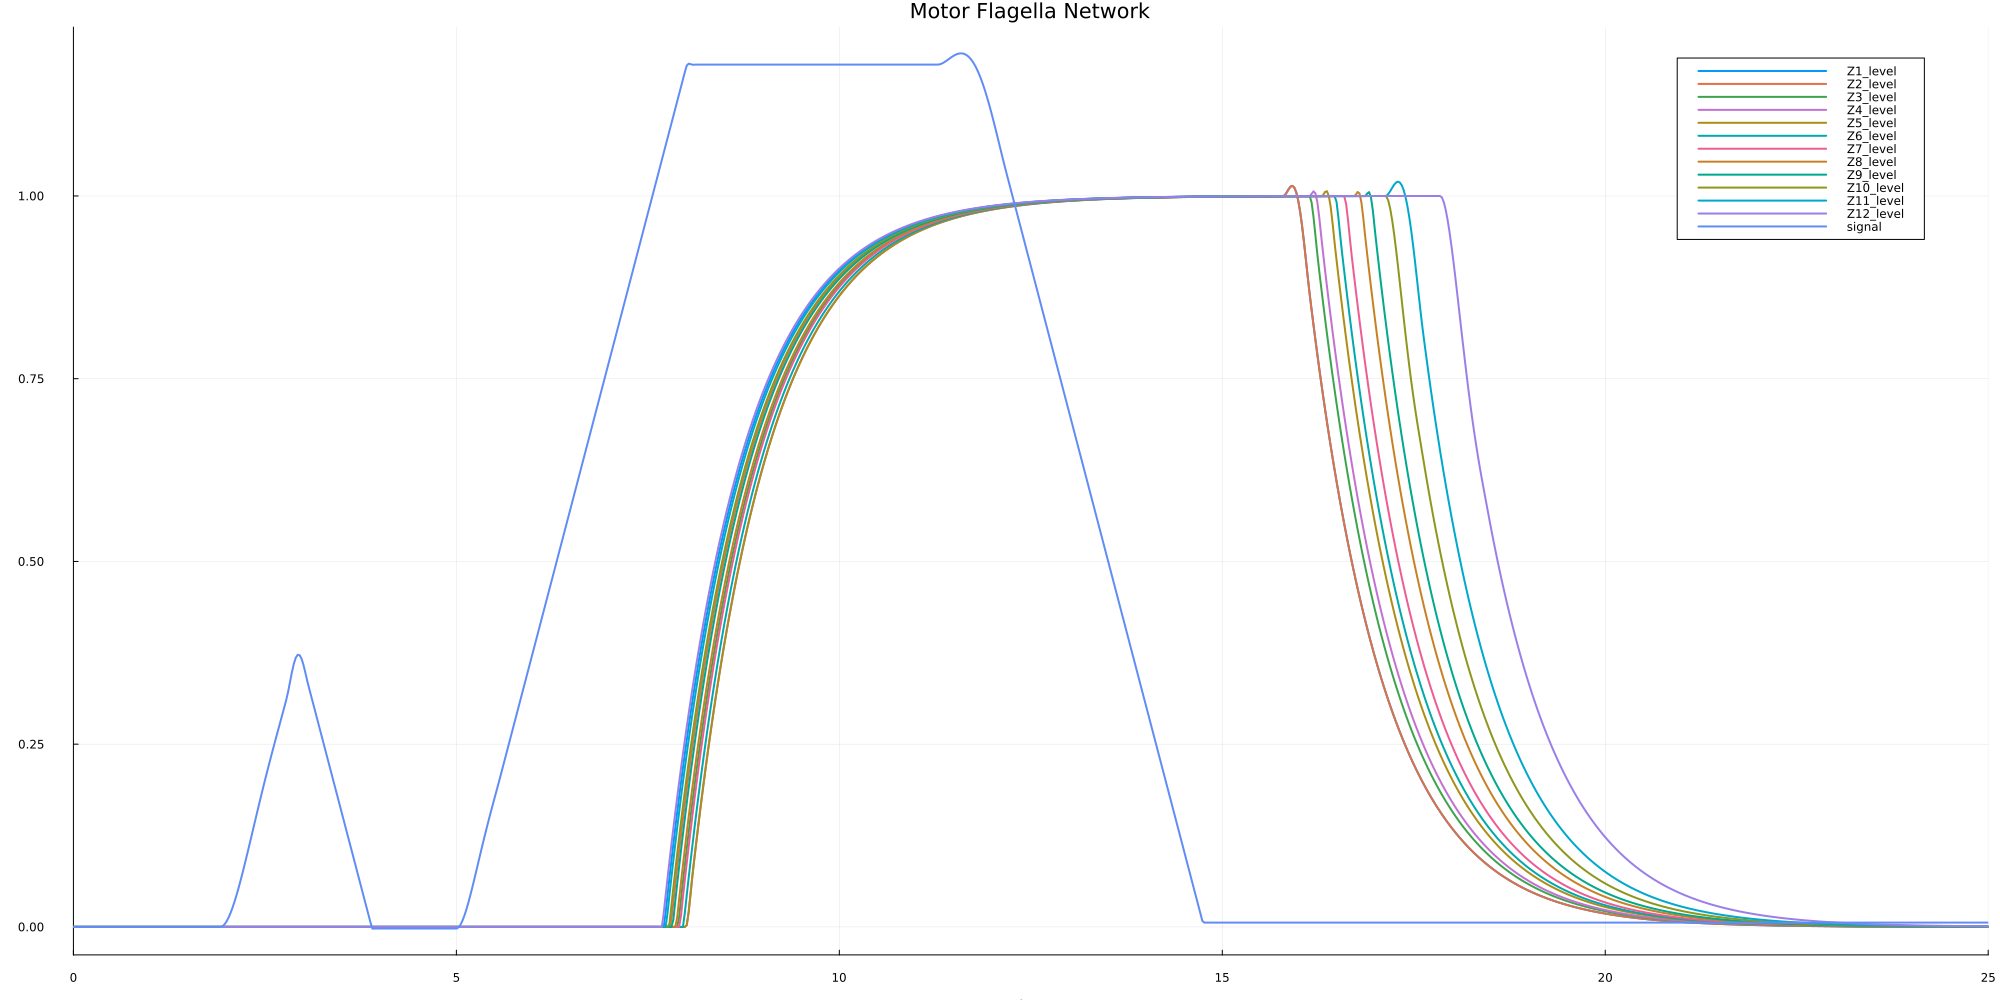
\includegraphics[width=650px, height=400px, angle=270]{motor_flagella.png}

\end{document}



